\chapter{Exams notes}

%------------------------------------------------------------------------%

\section{Ion implant range and +1 model}

Given an implant of an element with a dose Q and an energy E we can find form tables the values of 
    \begin{itemize}
    \item $R_p$ the projected range of our implant that is the maximum of our gaussian distribution that we expect
    \item $\Delta R_p$ the standard deviation of our gaussian distibution
    \end{itemize}
So we will have a distribution like 
\begin{equation}
C(x)=C_p exp\left(-\frac{(x-R_p)^2}{2\Delta R_p^2}\right)
\end{equation}
\\
where $C_p$ is the concentration at the peak of our distribution.\\
The total dose implanted will be $Q=\sqrt{2\pi\Delta R_p^2} C_p$ and so $C_p=\frac{Q}{\sqrt{2\pi\Delta R_p^2}}$ doing so we can write
\begin{equation}
C(x)=\frac{Q}{\sqrt{2\pi\Delta R_p^2}}exp\left(-\frac{(x-R_p)^2}{2\Delta R_p^2}\right)
\end{equation}
\\

If we want to know the dose that is present after a certain depth x
\begin{equation}
Q_{imp}=\int_x^{+\infty}C_p exp\left(-\frac{(x-R_p)^2}{2\Delta R_p^2}\right) dx
\end{equation}
That becomes 
\begin{equation}
Q_{imp}=\frac{Q}{2}erfc\left(\frac{x-R_p}{\sqrt{2}\Delta R_p}\right)
\end{equation}
\\
\vspace{5mm}

The function ercf has the following proprieties 
\begin{itemize}
\item ercf(x)=1-erf(x) if $x>0$
\item ercf(x)=1+erf(x) fi $x<0$
\end{itemize}

\vspace{6mm}

If we want to estimate the amount of interstitial caused by an implant using the +1 model we can say that the concentration of interstitial is equal to the dose Q implanted in silicon.\\
If the silicon is fully amorphised and than re-cristallized there are no interstital due to ion impantation since in an amorph cristal do not exists interstitials or defects.\\

%------------------------------------------------------------------------%

\section{Ion implant and dopant diffusion}

After an implant (with a certain dose Q and having also $R_p$ and $\Delta R_p$) there will always be a therma annealing process for a certain time t at a temperature T.\\
The profile of the doping will be a gaussian with the standard deviation modified by the diffusion due to thermal threatment so like

\begin{equation}
C(x)=\frac{Q_i}{\sqrt{2\pi (\Delta R_p^2+2Dt)}}exp\left(-\frac{(x-R_p)}{2(\Delta R_p^2+2Dt)}\right)
\end{equation} 
\\
From this we can know the concentration of dopants for all x.\\
Beware to correctrly set Q depending on the symmetry of the system.\\

%------------------------------------------------------------------------%

\section{CZ-growth}
CZ growth of silicon gives different doping concentrations for the wafers depending on the distance from the top of the ingot.\\
The parameters that we need to have the doping concentration at a certain value x are the segregation coefficient k and the initial dose of doping $C_0$
\begin{equation}
C=C_0 k (1-f)^{k-1}
\end{equation}
\\
where f is the \% of the ingot where we are.

\vspace{3mm}

Form the concentration we can derive the resistivity of the wafer as
\begin{equation}
\rho=\frac{1}{q\mu C}
\end{equation}

%------------------------------------------------------------------------%

\section{Deal-Grove model}
Using the correct tables parameters we can derive the coefficents B and B/A for wet or dry oxidation throught theyr Ahrrenius form 
\begin{equation}
B=C_1\cdot exp\left(-\frac{E_1}{kT} \right) \ \ \ \ \ \ \ \ \ \ \ \ B/A=C_2\cdot exp\left(-\frac{E_2}{kT} \right)
\end{equation}
or in an alternative way with theyr expressions
\begin{equation}
B=\frac{2DHP_G}{N} \ \ \ \ \ \ B/A=\frac{HP_G}{N \left( \frac{1}{k_s}+\frac{1}{h}  \right) }
\end{equation}
\\
remember that 
\begin{itemize}
\item B is related to the transport througth the present oxide so it isn't dependent on cristal orientation.
\item B/A is related to the interaction with the surface it's activation energy it's $\simeq 2eV$ that is the energy to break one Si-Si bond and it's strongly dependent on cristal orientation in fact
\begin{equation}
\left(\frac{B}{A}\right)_{<111>}=1.68\left(\frac{B}{A}\right)_{<100>}
\end{equation}
\end{itemize}
Notice that none of the mentioned parameters depends on pressure.\\

\vspace{5mm}

The model gives us the following expression
\begin{equation}
\frac{x^2}{B}+\frac{x}{B/A}=t+\tau
\end{equation}
\\
The boundary between the 2 regimes ,parabolic and linear, is given by the following thickness
\begin{equation}
x_b=\frac{B}{2B/A}
\end{equation}
\\
\vspace{5mm}

Beware that 46\% of the $SiO_2$ grows inside the silicon and the other 56\% over it.\\

%------------------------------------------------------------------------%

\section{Lito resoution limit}
Defining some parameters of our lito tool as:\\

\centering
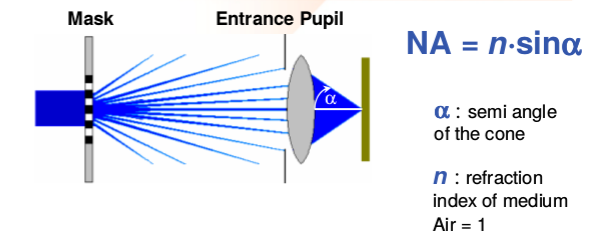
\includegraphics[width=0.5\textwidth]{NA.png}\\
\raggedright

NA determines the maximum number of diffraction orders that can be captured by projection lens and thus the quality of the reconstructed image.\\

\centering
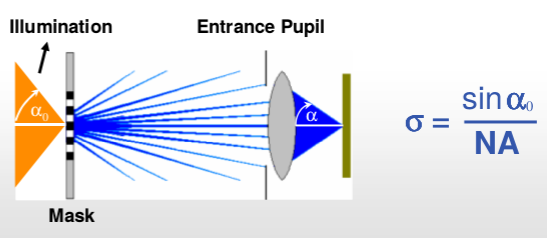
\includegraphics[width=0.5\textwidth]{sigma.png}\\
\raggedright

It defines the illumination of the mask, depends from source extension. For $\sigma=0$ we have coherent illumination $\sigma=1$ incoherent illumination.\\

\vspace{3mm}

For a coherent illumination that means a light perpendicular to the mask we have that the minimum resolution is 
\begin{equation}
R=\frac{1}{2}\frac{\lambda}{NA}
\end{equation}
\\
\vspace{3mm}

For a partially coherent illumination that means a light tilted by an angle $\theta$ the resolution is
\begin{equation}
R=\frac{1}{2}\frac{\lambda}{(1+\sigma)NA}
\end{equation}
\\

%------------------------------------------------------------------------%

\section{Lito contrast value}
Given a certain profile of aerial image the contrast value is 
\begin{equation}
C=\frac{I_{max}-I_{min}}{I_{max}+I_{min}}
\end{equation}
\\
With equal values of contrast it's better to choose the one with higher $I_{max}$





\section{Technology scaling; propagation delay}
Propagation delay of a metal wire can be modelled as
\begin{equation}
\tau\simeq 0.89 \cdot \varepsilon_{oxide}\varepsilon_0 \ \rho \  \frac{A}{F_{min}^2} 
\end{equation}
\\

%------------------------------------------------------------------------%

\section{Electromigration}
The critical lenght of the cluster can be expressed as 
\begin{equation}
L_{crit}=\frac{2\sigma_{crit}\Omega}{Z^*q\rho J}
\end{equation}
\\
Where $\Omega$ is the volume of the atom of metal and $\sigma_{crit}$ the value of the maximum stress.\\

%------------------------------------------------------------------------%

\section{Ion enanched etch rate}

Two process cooperating the ion etch and the byproducts deposition.\\
We can assume the number of deposited byproducts as
\begin{equation}
D=S_c(1-\theta)F_c
\end{equation}
\\
With $F_c$ flux of chemical species, $S_c$ sticking coefficient and (1-$\theta$) number of avabile sites.
The number of byproducts removed as
\begin{equation}
R=K_i\theta F_i
\end{equation}
\\
with $K_i$ sputtering efficency, $F_i$ flux of ionic species and $\theta$ number of occupied states.\\

In stationary conditions D=R so we can extract $\theta$ as
\begin{equation}
\theta=\frac{1}{1+\frac{K_iF_i}{S_cF_c}}
\end{equation}
so substituting this into the R expression we get the etch rate as 
\begin{equation}
E=\frac{1}{N}\left(\frac{1}{K_iF_i}+\frac{1}{S_cF_c}\right)
\end{equation}
\\
with N density of the material to be etched.\\

%------------------------------------------------------------------------%

\section{CVD regimes}

\centering
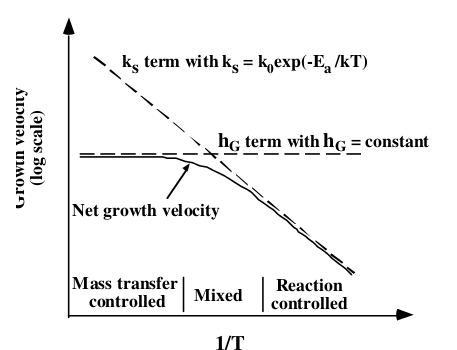
\includegraphics[width=0.5\textwidth]{CVD.png}\\
\raggedright

The velocity of deposition of a material in APCVD is determined by the slowest of two proces that operates in parallel; the transport of byproducts through the stagnant layer and the "reaction" with the surface.\\
The velocity can be mathematically described as 
\begin{equation}
v=\frac{k_sh_g}{k_s+h_g}\frac{C_T}{N}Y
\end{equation}
where $k_s$ is the chemical surface reaction rate (has an Ahrrenius form so strongly dependent on temperature) and $h_g$ the mass transport coefficient (indipendent form temperature).\\
We can distinguish in two case 
\begin{itemize}
\item $k_s<<h_g$ we are in surface reaction controlled regime; the geometry of the reaction does not matter so much this is the best case
\item $h_g<<k_s$ mass transport controlled regime; the geometry of the reactor is foundamental to control the stagnant layer 
\end{itemize}

\vspace{5mm}
We can increase the value of $h_g$ since we hope to stay in surface reaction controlled regime decreasing the value of the pressure since 
\begin{equation}
h_g=\frac{D_g}{\sigma_g}
\end{equation}
where $D_g$ is the diffusivity of the gas and $\sigma_g$ the stagnant layer thickness and $D_g\simeq 1/P$.\\








































